%!TEX root = ../thesis.tex
%*******************************************************************************
%****************************** Third Chapter **********************************
%*******************************************************************************
\chapter{METHODOLOGY}
\label{ch:methodology}

% **************************** Define Graphics Path **************************
\graphicspath{{Chapter3/Figs/Raster/}{Chapter3/Figs/PDF/}{Chapter3/Figs/Vector/}{Chapter3/Figs/}}

\section{Benchmark Reproduction and Experimental Foundation (FedSLD)}
\label{sec:fedsld_reproduction}

To establish a solid and fair baseline for our study, we begin by reproducing the benchmark from the FedSLD paper (Luo \& Wu, ISBI 2022) \cite{luo2022fedsld}. FedSLD is a well-known federated learning study designed specifically for medical image classification under non-IID data distributions. In this section, we describe the datasets, the non-IID partitioning method, the experimental configuration, the foundational baseline algorithms (FedAvg and FedProx), and the reproduced benchmark results.

\subsection{Benchmark Datasets: Focus on PathMNIST and OrganAMNIST}
The MedMNIST v2 collection \cite{yang2023medmnist} provides standardized 2D biomedical image datasets for machine learning research. While the collection includes several datasets (such as BloodMNIST and DermaMNIST), this research focuses primarily on two representative benchmarks:
\begin{enumerate}
    \item \textbf{PathMNIST}: A dataset of colon pathology images containing 9 diagnostic classes (such as adipose, debris, lymphocytes, and tumor epithelium). It exhibits significant variations in tissue textures and histological staining.
    \item \textbf{OrganAMNIST}: A dataset of abdominal CT organ patches featuring 11 anatomical classes (such as liver, kidneys, spleen, and bladder). It presents subtle grayscale differences across diverse organs.
\end{enumerate}
Other datasets in the collection, such as BloodMNIST (blood cell classification) and DermaMNIST (dermatoscopy skin lesion screening), are also supported in our codebase, but PathMNIST and OrganAMNIST serve as the core evaluation benchmarks in this thesis.

\subsection{Data Partitioning: Practical versus Pathological Non-IID}
In the FedSLD benchmark \cite{luo2022fedsld}, the authors evaluate federated learning under two distinct non-IID partitioning schemes:
\begin{itemize}
    \item \textbf{Pathological Non-IID}: Originally introduced in the foundational FedAvg paper \cite{mcmahan2017communication}, this classic scheme artificially restricts each client to hold samples from only a few classes (for example, exactly 2 classes per hospital). While it creates extreme label skew to test theoretical convergence, it is unrealistic in healthcare because actual hospitals treat a diverse spectrum of diseases, rather than just one or two specific conditions.
    \item \textbf{Practical Non-IID}: To overcome the artificial nature of the pathological split, FedSLD \cite{luo2022fedsld} designed the Practical partition, which reflects clinical reality much more accurately. In real-world healthcare collaborations, medical institutions differ substantially in size, patient volume, and diagnostic specialization.
\end{itemize}

Specifically, for $K = 12$ clients, the Practical partition applies clinical proportions \textbf{independently for each individual class}, rather than as a single global split across the entire dataset:
\begin{itemize}
    \item For every diagnostic category, the samples belonging to that class are divided into 12 shards: one dominant shard containing \textbf{80\%} of the class samples, one medium shard containing \textbf{10\%}, and ten small shards sharing the remaining \textbf{10\%} equally (\textbf{1\%} each).
    \item These shards are then randomly assigned across the 12 clients for each class.
\end{itemize}

As a result of this per-class sharding mechanism, a single client can be assigned the 80\% dominant shard for multiple disease categories. This accurately simulates large specialized medical centers that receive a high volume of cases across several related conditions (for instance, in PathMNIST, one large client holds the 80\% dominant shards for three different classes, totaling over 26,000 samples). Meanwhile, other clients receive only small 1\% shards across all classes (simulating small local clinics with under 900 samples). This partitioning strategy creates realistic volume disparities (a $\sim$29$\times$ sample count difference between the largest and smallest clients) alongside natural clinical specialization, while guaranteeing that all clients retain at least a baseline number of samples for every class.


\subsection{Baseline Algorithms: FedAvg and FedProx}
To evaluate model performance, we implement and reproduce two foundational federated learning algorithms:
\begin{enumerate}
    \item \textbf{FedAvg (Federated Averaging)} \cite{mcmahan2017communication}: The classic baseline algorithm. In each round, the central server sends the current global model to the clients. Each client trains the model on its local data using SGD and sends the updated weights back. The server then computes a weighted average of these weights based on each client's sample count:
    \begin{equation}
        w^{(r+1)} = \sum_{k=1}^K \frac{n_k}{N} w_k^{(r+1)}
        \label{eq:fedavg_simple}
    \end{equation}
    When data across clients is heavily non-IID, local models tend to move toward their local optima, causing the global model to suffer from \textit{client drift}.

    \item \textbf{FedProx (Federated Proximal)} \cite{li2020federated}: An extension of FedAvg designed to improve stability under heterogeneity. FedProx adds a proximal regularization term to each client's local loss function:
    \begin{equation}
        \min_{w} \mathcal{L}_k(w) = F_k(w) + \frac{\mu}{2} \|w - w^{(r)}\|^2
        \label{eq:fedprox_simple}
    \end{equation}
    where $\mu > 0$ is a proximal penalty parameter (we use $\mu = 0.01$). This term keeps local model updates closer to the global model $w^{(r)}$, helping to reduce client drift.
\end{enumerate}

\subsection{Experimental Configuration}
To reproduce the FedSLD benchmark faithfully and ensure fair comparisons, we adopt the exact experimental parameters specified in the FedSLD paper:
\begin{itemize}
    \item \textbf{Number of Clients}: $K = 12$ clients participating in federated training.
    \item \textbf{Communication Rounds}: 80 rounds.
    \item \textbf{Local Epochs}: 5 local epochs per client in each round.
    \item \textbf{Mini-Batch Size}: 256.
    \item \textbf{Optimizer}: Stochastic Gradient Descent (SGD) with momentum $\mu = 0.9$ and weight decay $10^{-4}$.
    \item \textbf{Learning Rate}: Initial learning rate $\eta = 0.01$ (with a fixed schedule across rounds).
    \item \textbf{Network Architecture}: In their implementation details, Luo \& Wu \cite{luo2022fedsld} specify: \textit{``We use the classic four-layer CNN model with two $5\times 5$ convolutional layers and two fully connected layers (hidden layer has 500 units)''}, following the standard federated benchmark model established by McMahan et al. \cite{mcmahan2017communication}. This architecture comprises $\sim$570k parameters and operates without Batch Normalization layers.
\end{itemize}

Importantly, for our proposed method, we maintain this exact experimental configuration and strictly follow the partitioning design of the original paper---dividing each class into 12 shards according to the 80\%--10\%--1\% clinical proportions. This guarantees that all subsequent performance comparisons and gains stem directly from algorithmic improvements rather than different hyper-parameters or altered partition settings.

\subsection{Reproduction Results and Baseline Selection}
\label{subsec:repro_results_baseline}

Table~\ref{tab:fedsld_repro_comparison} compares the original results published in the FedSLD paper \cite{luo2022fedsld} against our reproduction across both PathMNIST and OrganAMNIST under the Practical non-IID partition. For our reproduction, we report the mean and standard deviation across independent runs. We evaluate performance using the two official FedSLD metrics:
\begin{itemize}
    \item \textbf{BMCTA (Best Mean Client Test Accuracy)}: The average test accuracy computed across each of the 12 individual client local test sets.
    \item \textbf{BTA (Best Total Accuracy)}: The overall test accuracy evaluated on the pooled global test set.
\end{itemize}

\begin{table}[htbp]
\centering
\small
\setlength{\tabcolsep}{4.5pt}
\caption{Benchmark results under Practical Non-IID partition (12 clients, 80 rounds) compared with original FedSLD paper and Centralized Upper Bound.}
\label{tab:fedsld_repro_comparison}
\begin{tabular}{llcccc}
\toprule
\multirow{2}{*}{\textbf{Dataset}} & \multirow{2}{*}{\textbf{Method / Algorithm}} & \multicolumn{2}{c}{\textbf{FedSLD Paper \cite{luo2022fedsld}}} & \multicolumn{2}{c}{\textbf{Our Reproduction}} \\
\cmidrule(lr){3-4} \cmidrule(lr){5-6}
& & \textbf{BMCTA (\%)} & \textbf{BTA (\%)} & \textbf{BMCTA (\%)} & \textbf{BTA (\%)} \\
\midrule
\multirow{4}{*}{OrganAMNIST} & Centralized (Upper Bound) & --- & --- & $81.99 \pm 0.84$ & $81.99 \pm 0.84$ \\
                             & FedAvg                    & $82.32$ & $85.69$ & $82.39 \pm 0.84$ & $82.98 \pm 0.85$ \\
                             & FedProx                   & $81.53$ & $85.54$ & $82.29 \pm 0.81$ & $82.88 \pm 0.84$ \\
                             & FedSLD (Paper Method)     & $84.75$ & $87.37$ & --- & --- \\
\midrule
\multirow{4}{*}{PathMNIST}    & Centralized (Upper Bound) & --- & --- & $77.11 \pm 1.33$ & $77.11 \pm 1.33$ \\
                             & FedAvg                    & $52.70$ & $57.38$ & $77.76 \pm 2.05$ & $79.44 \pm 1.26$ \\
                             & FedProx                   & $52.77$ & $57.72$ & $77.99 \pm 1.93$ & $79.75 \pm 0.76$ \\
                             & FedSLD (Paper Method)     & $53.87$ & $57.90$ & --- & --- \\
\bottomrule
\end{tabular}
\end{table}

Table~\ref{tab:fedsld_repro_comparison} reveals several key empirical insights across the benchmarks:
\begin{enumerate}
    \item \textbf{OrganAMNIST Consistency and Discrepancy}: On OrganAMNIST, our reproduced client-average test accuracy (BMCTA) matches the published paper remarkably well ($82.39\%$ vs. $82.32\%$ for FedAvg). However, the global pooled test accuracy (BTA) achieved by our reproduction ($82.98\%$) is approximately $2.7\%$ lower than the value reported in the original paper ($85.69\%$).
    \item \textbf{PathMNIST Accuracy}: On PathMNIST, our reproduced models achieve substantially higher accuracy ($\approx 79.4\%$ BTA) than the relatively low numbers reported in the FedSLD paper ($\approx 57.4\%$ BTA).
    \item \textbf{Federated vs. Centralized Gap}: As expected in non-IID federated learning, distributed training suffers from performance degradation compared to centralized training. The extreme sample imbalance in the Practical partition (where small clinics hold only 1\% of samples per class) causes client drift that prevents FedAvg and FedProx from reaching centralized performance levels.
\end{enumerate}

\paragraph{Discussion and Analysis of Reproduction Discrepancies.}
In experimental reports and scientific evaluations, addressing numerical differences between published literature and independent reproductions is essential. We attribute the observed performance gap on OrganAMNIST and PathMNIST to three fundamental factors:
\begin{itemize}
    \item \textbf{Absence of Public Random Seeds}: The authors of FedSLD \cite{luo2022fedsld} did not release the exact random seed used for their dataset splitting or weight initialization. In the Practical non-IID partitioning scheme, each class is divided into 12 shards ($1 \times 80\%$, $1 \times 10\%$, $10 \times 1\%$) and randomly shuffled across clients. Because shard assignment is stochastic, different seeds produce drastically different client compositions. For example, if a random seed assigns the 80\% dominant shards of several classes to a single client, that client becomes an overwhelming outlier, exacerbating client drift and lowering global convergence.
    \item \textbf{Non-Convex Optimization and Weight Initialization}: Deep neural networks trained in decentralized, non-IID settings are highly sensitive to initial parameter values. Different initializations cause local SGD trajectories to diverge into different local minima, leading to a natural variation of $2\% - 3\%$ across independent trials.
    \item \textbf{Unspecified Training Details}: Minor implementation nuances—such as mini-batch shuffling order, exact learning rate decay milestones, and gradient clipping thresholds—were not documented in the original publication, contributing to empirical variance.
\end{itemize}

\paragraph{Establishing Our Reproduction as the Fair Baseline.}
Rather than viewing these variations as a limitation, this discrepancy reinforces the necessity of establishing our own rigorous, fully documented benchmark. Directly comparing our subsequent proposed methodology against numbers from an un-seeded, non-reproducible external baseline would be scientifically invalid and unfair. 

Therefore, we adopt our own reproduced results (evaluated over 5 independent runs with fixed random seeds and identical training pipelines) as the authoritative, consistent baseline. Any performance improvements demonstrated by our proposed Dual-Heterogeneity strategy in Chapter~\ref{ch:experiments_results} are evaluated on this exact same data partition and baseline foundation, guaranteeing a strictly fair and credible comparison.

\section{Proposed Dual-Heterogeneity Method}
\label{sec:proposed_method}

Having established a solid and reproducible baseline in Section~\ref{sec:fedsld_reproduction}, this section introduces our proposed federated learning framework. We design a unified strategy that addresses two major hurdles in decentralized healthcare AI: dual heterogeneity (feature shift and client drift) and edge resource constraints.

\subsection{Motivation and Dual Heterogeneity Challenges}
\label{subsec:motivation_dual_heterogeneity}

In real-world medical federated networks, data heterogeneity manifests in two distinct, orthogonal dimensions:
\begin{enumerate}
    \item \textbf{Feature/Domain Shift}: Different hospitals and medical centers utilize varying imaging equipment, scanning protocols, radiation dosages, and histological staining techniques. As a result, the input features (such as pixel intensities, texture patterns, and color distributions) differ across institutions even for identical anatomical structures or disease conditions.
    \item \textbf{Client Drift from Label and Volume Imbalance}: Participating clinical sites naturally differ in patient volume and medical specialization. In the Practical non-IID partition (as detailed in Section~\ref{sec:fedsld_reproduction}), a large medical center may hold 80\% of the cases for several disease categories, while smaller clinics hold only 1\% shards. Under standard federated averaging (FedAvg), local model updates from smaller or specialized clients quickly drift toward their local optima, causing destructive interference during global aggregation.
\end{enumerate}

Existing methods typically address only one of these two issues:
\begin{itemize}
    \item \textbf{FedBN} \cite{li2021fedbn} effectively mitigates feature shift by preserving local Batch Normalization layers, but it does not prevent client drift caused by extreme label distribution skew.
    \item \textbf{SCAFFOLD} \cite{karimireddy2020scaffold} corrects client drift using control variates, but it assumes that all clients share identical feature representations and does not account for domain-level scanner variations.
\end{itemize}

Moreover, the classic baseline CNN architecture used in the original FedSLD paper \cite{luo2022fedsld} ($\sim$570k parameters) does not incorporate any normalization layers. Without normalization mechanisms, it is fundamentally impossible to isolate client-specific scanner variations from shared semantic representations via techniques like FedBN.

To overcome these combined bottlenecks while maintaining strict comparability with the baseline, we propose a synergistic framework that augments the \textbf{classic 4-layer CNN architecture ($\sim$570k parameters) with Batch Normalization layers} and applies a \textbf{Dual-Heterogeneity strategy (FedBN + SCAFFOLD)} featuring \textbf{Zero-Drift Masking} and \textbf{decoupled post-step updates}.

\subsection{Model Architecture: BatchNorm-Augmented CNN (~570k Parameters)}
\label{subsec:lightweight_architecture}

To ensure an exact and fair comparison with the FedSLD baseline, our proposed framework preserves the identical backbone capacity and layer dimensions of the classic 4-layer CNN, but integrates Batch Normalization (\texttt{BatchNorm2d}) immediately following each convolutional layer.

The detailed layer specifications of our BatchNorm-augmented model (\texttt{BaselineBN}) are:
\begin{enumerate}
    \item \textbf{Convolutional Block 1}: A $5 \times 5$ 2D convolution layer with 32 filters (stride = 1, padding = 0), followed by Batch Normalization (\texttt{BatchNorm2d}(32)), a ReLU activation function, and a $2 \times 2$ Max-Pooling layer with stride 2. This reduces the spatial resolution from $28 \times 28 \to 24 \times 24 \to 12 \times 12$.
    \item \textbf{Convolutional Block 2}: A $5 \times 5$ convolution increasing channels from 32 to 64 (stride = 1, padding = 0), followed by \texttt{BatchNorm2d}(64), ReLU, and $2 \times 2$ Max-Pooling (stride 2), reducing spatial size from $12 \times 12 \to 4 \times 4$.
    \item \textbf{Dense Hidden Layer}: The resulting $64 \times 4 \times 4 = 1024$ flattened tensor is projected through a fully connected layer with 500 hidden units ($\text{Linear}(1024, 500)$), followed by a ReLU activation.
    \item \textbf{Classification Head}: A final linear projection layer mapping the 500 hidden features directly to class logits ($\text{Linear}(500, C)$, where $C$ is the number of classes, e.g., 9 for PathMNIST and 11 for OrganAMNIST).
\end{enumerate}

Table~\ref{tab:model_architecture_comparison} and Fig.~\ref{fig:model_architecture_comparison} present a direct structural comparison between the un-normalized FedSLD baseline CNN and our BatchNorm-augmented CNN.

\begin{figure}[htbp]
\centering
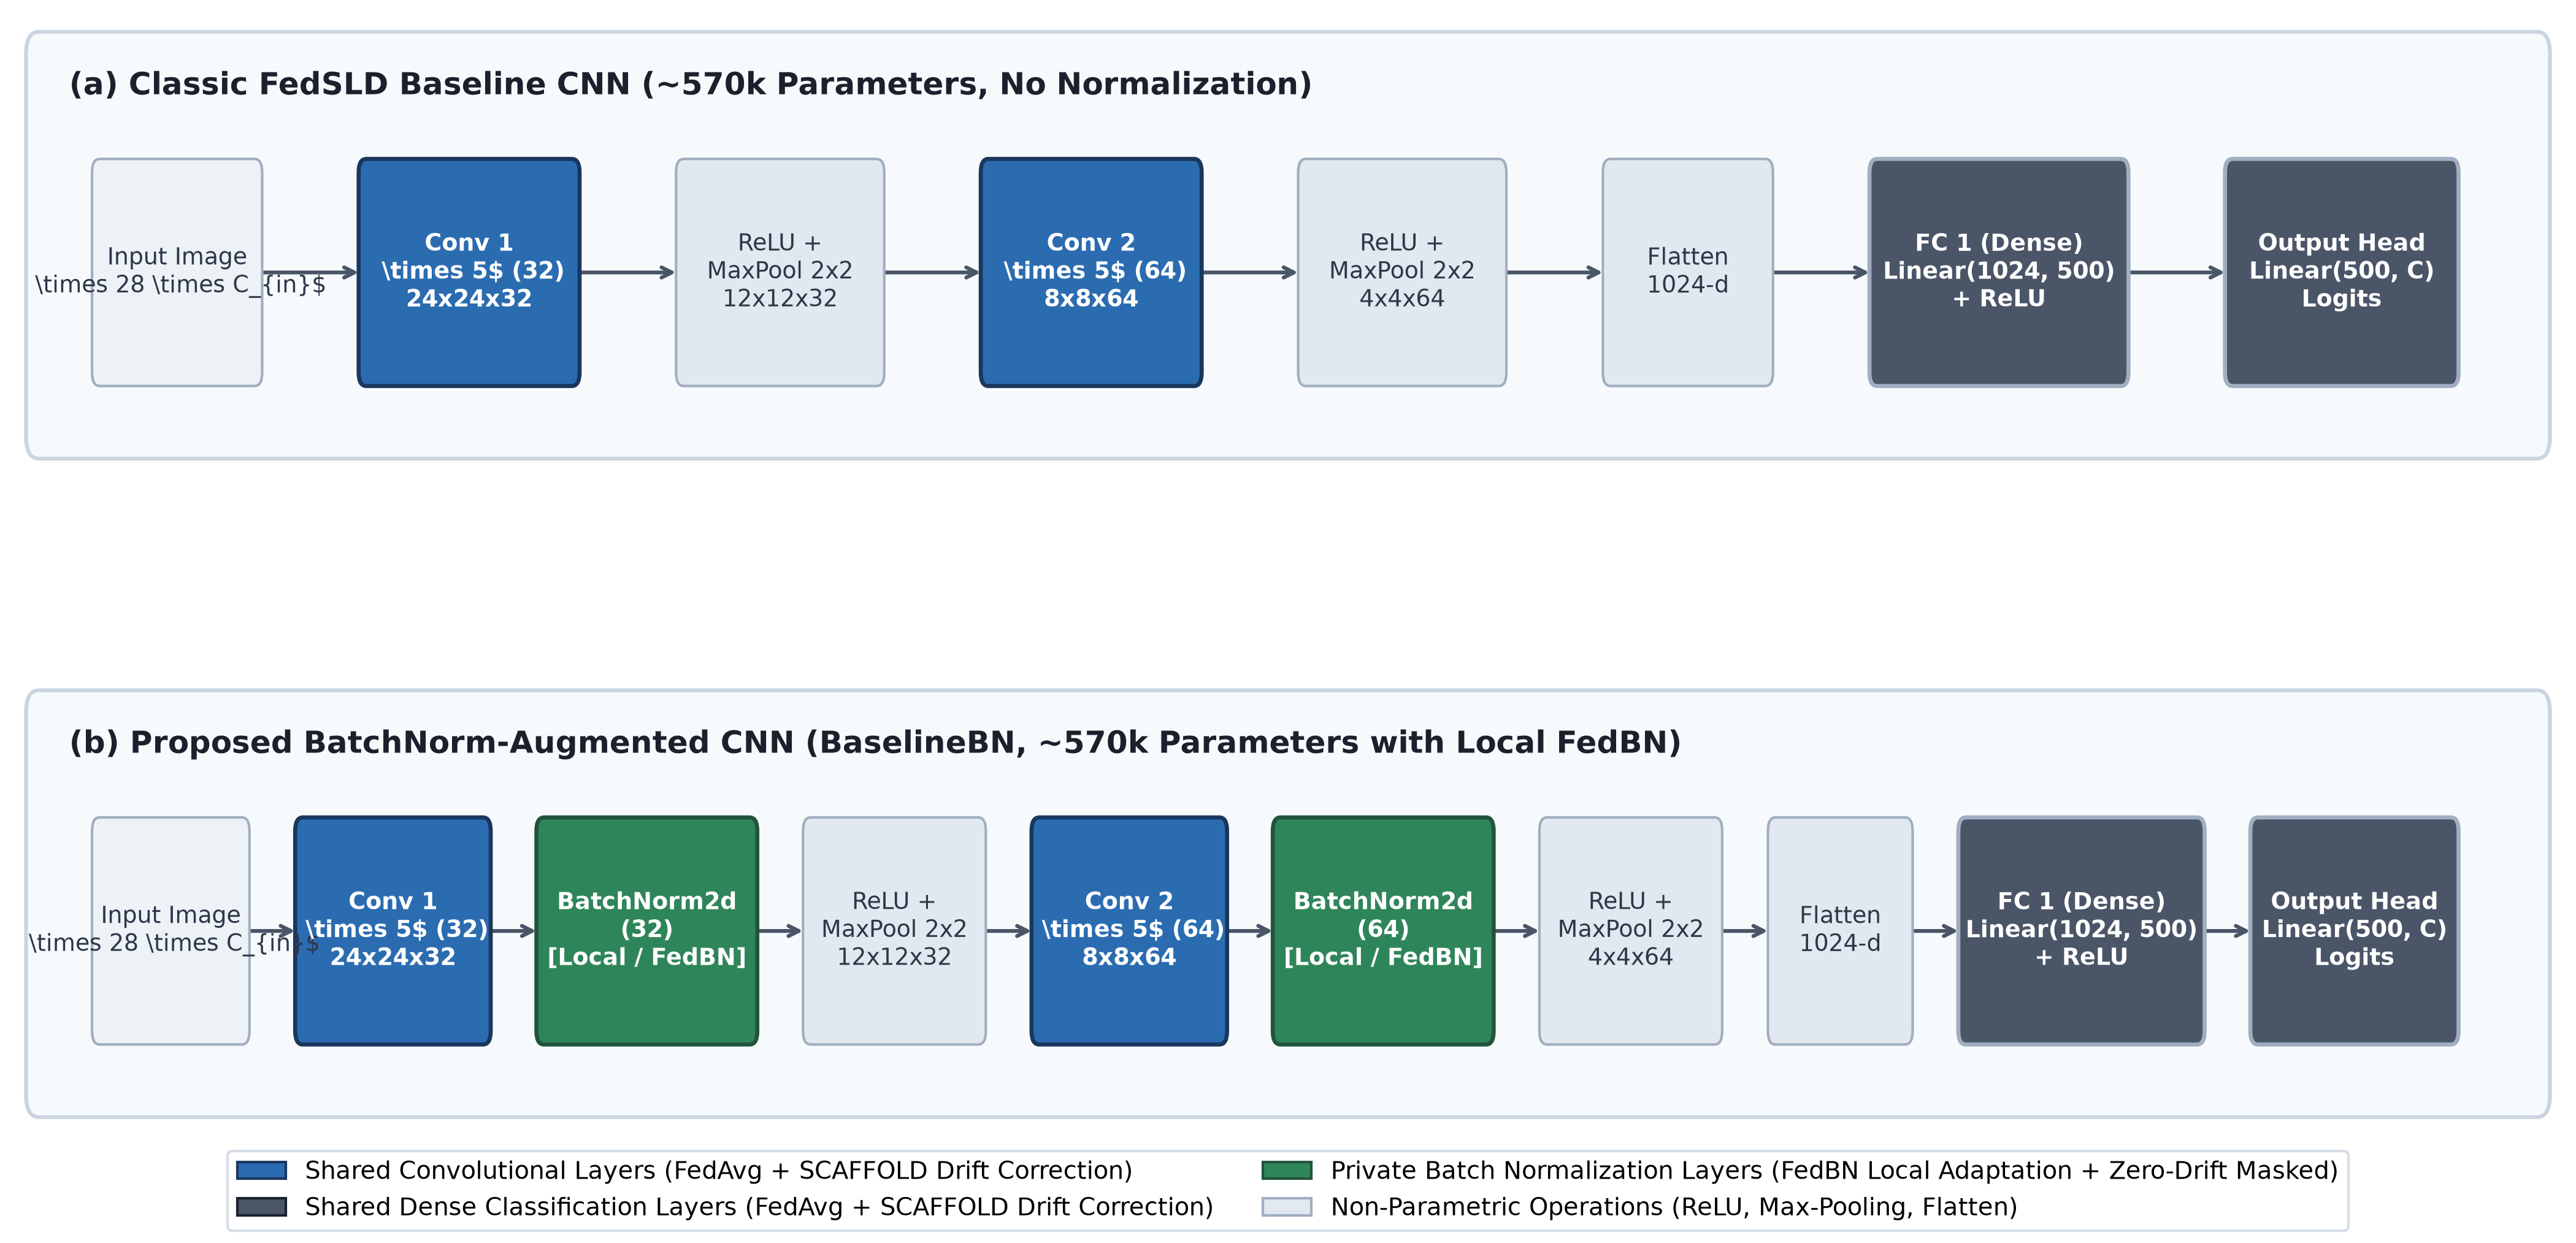
\includegraphics[width=\textwidth]{Chapter3/Figs/Raster/model_architecture_comparison.png}
\caption{Architectural comparison between (a) the classic un-normalized 4-layer CNN from the FedSLD paper \cite{luo2022fedsld}, and (b) our proposed BatchNorm-augmented CNN (\texttt{BaselineBN}). In our proposed method, the convolutional filters and dense classification layers (blue and dark gray) are aggregated globally with SCAFFOLD drift correction, whereas the Batch Normalization layers (green) are kept strictly local to each client hospital (FedBN) and masked from drift correction ($M_l = 0$).}
\label{fig:model_architecture_comparison}
\end{figure}

\begin{table}[htbp]
\centering
\small
\setlength{\tabcolsep}{4.5pt}
\caption{Architectural comparison between classic baseline CNN and our BatchNorm-augmented model.}
\label{tab:model_architecture_comparison}
\begin{tabular}{lcc}
\toprule
\textbf{Layer / Component} & \textbf{Baseline CNN \cite{luo2022fedsld}} & \textbf{Proposed Model (BaselineBN)} \\
\midrule
Conv Block 1 & $5 \times 5$ Conv, 32 + ReLU + Pool & $5 \times 5$ Conv, 32 + \textbf{BN} + ReLU + Pool \\
Conv Block 2 & $5 \times 5$ Conv, 64 + ReLU + Pool & $5 \times 5$ Conv, 64 + \textbf{BN} + ReLU + Pool \\
Dense Layer & Linear($1024 \to 500$) + ReLU & Linear($1024 \to 500$) + ReLU \\
Output Layer & Linear($500 \to C$) & Linear($500 \to C$) \\
Total Parameters & $\sim 570\text{k}$ ($570,705$ on PathMNIST) & $\sim 570\text{k}$ ($570,897$ on PathMNIST) \\
Parameter Delta & Baseline ($0$ BN params) & $+192$ BN params ($< 0.04\%$) \\
\bottomrule
\end{tabular}
\end{table}

As shown in Table~\ref{tab:model_architecture_comparison}, adding Batch Normalization introduces merely 192 additional parameters (comprising affine weights and biases for the 32 and 64 feature maps), representing less than a $0.04\%$ change in total model size. Consequently, the feature representation capacity and memory footprint remain virtually identical to the original FedSLD baseline ($\sim$570k parameters). This design ensures that any performance improvements achieved by our proposed method arise strictly from algorithmic advancements (FedBN domain adaptation and SCAFFOLD drift correction) rather than differences in model scale.

\subsection{Handling Domain Shift via Local Batch Normalization (FedBN)}
\label{subsec:fedbn_formulation}

Batch Normalization layers standardize layer inputs using the mean $\mu_B$ and variance $\sigma_B^2$ computed across mini-batch $B$, followed by learnable affine parameters (scale $\gamma$ and shift $\beta$):
\begin{equation}
    \hat{x} = \frac{x - \mu_B}{\sqrt{\sigma_B^2 + \epsilon}}, \quad y = \gamma \hat{x} + \beta
    \label{eq:batchnorm}
\end{equation}
During training, the layer also maintains exponential running statistics ($\mu_{\text{run}}, \sigma_{\text{run}}^2$) to approximate the global feature distribution for inference.

In standard federated aggregation (such as FedAvg), all parameters—including Batch Normalization statistics—are averaged across clients. However, when different hospitals use different scanners and staining techniques, averaging these parameters forces every client to adopt a blurred, contradictory feature representation, degrading local accuracy.

Following the principles of FedBN \cite{li2021fedbn}, our framework partitions the model parameters into two distinct subsets:
\begin{enumerate}
    \item \textbf{Global Shared Parameters} ($\Theta_{\text{global}}$): The weights and biases of convolutional filters and the final classification head ($W_{\text{conv}}, W_{\text{fc}}$). These capture general visual representations and semantic category boundaries, and are aggregated by the central server.
    \item \textbf{Local Private Parameters} ($\Theta_{\text{local}}$): All Batch Normalization parameters ($\gamma, \beta$) and running statistics ($\mu_{\text{run}}, \sigma_{\text{run}}^2$). These parameters remain strictly on each local client and are never uploaded to the server or averaged.
\end{enumerate}

By keeping Batch Normalization local, each hospital client standardizes internal activations according to its specific imaging distribution, harmonizing domain differences while collaboratively benefiting from shared representation learning.

\subsection{Correcting Client Drift via SCAFFOLD with Zero-Drift Masking}
\label{subsec:scaffold_drift_correction}

While local Batch Normalization resolves domain discrepancies, it does not alleviate the severe gradient bias induced by label and sample volume disparities. To prevent local models from drifting away from the global optimum, our framework incorporates control variates based on SCAFFOLD \cite{karimireddy2020scaffold}, enhanced with two critical adaptations: \textbf{Zero-Drift Masking} and \textbf{Decoupled Post-Step Updates}.

\subsubsection{Control Variate Formulation}
In SCAFFOLD, the server maintains a global control variate $c$, and each client $i$ maintains a local control variate $c_i$. The control variate $c_i$ estimates the average update direction of client $i$, while $c$ represents the consensus update direction across the federation. 

During local training, client $i$ corrects its local gradient $g_i(w)$ by applying the drift difference $(c - c_i)$:
\begin{equation}
    \tilde{g}_i(w) = g_i(w) - c_i + c
    \label{eq:scaffold_drift_grad}
\end{equation}
If client $i$ receives a disproportionate number of samples from a single class, its local gradient $g_i(w)$ pulls the weights strongly toward that class. The term $- c_i + c$ counteracts this local bias and steers the trajectory back toward the global objective.

\subsubsection{Zero-Drift Masking for BatchNorm Layers}
A key technical novelty in our framework is the interaction between FedBN and SCAFFOLD. Because Batch Normalization parameters are deliberately kept private to preserve client-specific domain adaptation, applying global control variate correction to BN parameters would counteract their local specialization.

To maintain algorithmic harmony, we implement a \textbf{Zero-Drift Mask} $M \in \{0, 1\}^{|\Theta|}$:
\begin{equation}
    M_l = \begin{cases}
        0, & \text{if parameter } l \text{ belongs to a BatchNorm layer}, \\
        1, & \text{otherwise (convolutional and linear weights)}.
    \end{cases}
    \label{eq:zero_drift_mask}
\end{equation}
The effective drift correction applied to layer $l$ is governed by:
\begin{equation}
    \Delta_{\text{drift}, l} = M_l \cdot (c_l - c_{i, l})
    \label{eq:masked_drift}
\end{equation}
This ensures that non-BN layers receive full drift correction across heterogeneous label distributions, while BN layers remain unperturbed to adapt freely to local scanner characteristics.

\subsubsection{Decoupled Post-Step Parameter Update}
In standard federated implementations, the correction term is often added directly into the gradient tensor prior to optimizer stepping ($g \leftarrow g + c - c_i$). However, as observed in production frameworks such as NVIDIA FLARE \cite{roth2022nvidia}, injecting drift directly into the gradient corrupts the momentum velocity buffers in SGD (when momentum $\beta > 0$) or the first and second moment vectors in Adam. Over multiple local epochs, this momentum pollution leads to numerical instability and divergence.

To resolve this issue, we decouple the drift correction from the optimizer. For each mini-batch step, client $i$ first performs standard backpropagation and optimizer updating:
\begin{equation}
    w \leftarrow \text{OptimizerStep}\big(w, \, \nabla \mathcal{L}(w; \mathcal{B})\big)
    \label{eq:optimizer_step}
\end{equation}
Immediately following the optimizer step, the masked drift correction is applied directly to the parameter tensor without gradient tracking:
\begin{equation}
    w \leftarrow w - \eta \cdot \Delta_{\text{drift}}
    \label{eq:decoupled_step}
\end{equation}
where $\eta$ is the current local learning rate. This decoupled update guarantees exact mathematical drift compensation while maintaining clean momentum buffers across varying optimizers and learning rate schedules.

\subsection{Federated Workflow and Lifecycle}
\label{subsec:federated_workflow}

The complete execution lifecycle of our proposed framework across communication rounds proceeds through the following sequential stages:

\begin{enumerate}
    \item \textbf{Server Broadcast (Round $r$)}:
    The central server broadcasts the current global model weights $w_{\text{global}}^{(r)}$ (covering non-BN parameters) and the global control variate $c^{(r)}$ to all participating clients $i \in \{1, \dots, K\}$.

    \item \textbf{Local Initialization}:
    Client $i$ receives $w_{\text{global}}^{(r)}$ and loads these weights into its local model while retaining its local Batch Normalization parameters ($\gamma_i, \beta_i, \mu_{i, \text{run}}, \sigma_{i, \text{run}}^2$).

    \item \textbf{Local Training with Decoupled Drift}:
    Client $i$ trains for $E$ local epochs over its private dataset $\mathcal{D}_i$. For each mini-batch, the client executes the standard optimizer step and immediately applies the masked drift update $- \eta \cdot M \cdot (c^{(r)} - c_i^{(r)})$.

    \item \textbf{Local Control Variate Update}:
    At the conclusion of local training, client $i$ computes its updated local control variate $c_i^{(r+1)}$ following SCAFFOLD Option~2:
    \begin{equation}
        c_i^{(r+1)} = c_i^{(r)} - c^{(r)} + \frac{1}{K_{\text{steps}} \cdot \eta} \big(w_{\text{global}}^{(r)} - w_i^{(r+1)}\big)
        \label{eq:client_c_update}
    \end{equation}
    where $K_{\text{steps}}$ is the total number of local gradient steps taken. The client then computes the control variate delta $\Delta c_i = c_i^{(r+1)} - c_i^{(r)}$.

    \item \textbf{Client Upload}:
    Client $i$ sends only its updated trainable non-BN weights $w_i^{(r+1)}$ and control variate delta $\Delta c_i$ back to the server. Local BN parameters remain private on the device.

    \item \textbf{Server Aggregation}:
    The server aggregates the received non-BN parameters using sample-weighted averaging, and updates the global control variate:
    \begin{align}
        w_{\text{global}}^{(r+1)} &= \sum_{i=1}^K \frac{n_i}{N} w_i^{(r+1)} \label{eq:server_agg_w} \\
        c^{(r+1)} &= c^{(r)} + \frac{1}{K} \sum_{i=1}^K \Delta c_i \label{eq:server_agg_c}
    \end{align}
    where $n_i = |\mathcal{D}_i|$ and $N = \sum_{i=1}^K n_i$.
\end{enumerate}

By unifying the standard $\sim$570k CNN architecture with private local Batch Normalization (FedBN) and masked decoupled control variates (SCAFFOLD), our proposed framework simultaneously addresses domain shifts and client drift without altering the fundamental model scale. Detailed empirical validations, comparisons against other FL strategies, and ablation studies are presented in Chapter~\ref{ch:experiments_results}.
